\documentclass[11pt, a4paper]{article}

\usepackage[utf8]{inputenc}
\usepackage[spanish]{babel}
\usepackage{amsmath}
\usepackage{amsfonts}
\usepackage{amssymb}
\usepackage{graphicx}
\usepackage{svg}
\usepackage{circuitikz}
\usepackage{booktabs}
\usepackage{geometry}
\usepackage{hyperref}
\usepackage{float}
\usepackage{xcolor}
\usepackage{siunitx}

\geometry{top=2.5cm, bottom=2.5cm, left=2.5cm, right=2.5cm}

\title{\textbf{Reporte Técnico de Diseño: Amplificador de Instrumentación de Ultra Precisión (SupOpAmp)}}
\author{Ingeniería de Diseño Analógico}
\date{\today}

\begin{document}

\maketitle

\begin{abstract}
Este documento detalla la arquitectura, análisis matemático, y validación espectral de un amplificador de instrumentación de ultra alta precisión basado en una topología compuesta denominada \textbf{SupOpAmp}. El sistema está diseñado para ofrecer una ganancia exacta de $20,000$ ($86\text{ dB}$), manteniendo un ancho de banda superior a los $500\text{ kHz}$, y proveyendo control de impedancias y capacidades de salida de alta potencia ($50\,\Omega$) a través de un diseño iterativo asistido por simulación SPICE de última generación.
\end{abstract}

\tableofcontents
\newpage

\section{Arquitectura y Topología del Circuito}

El amplificador de instrumentación está fundamentado en la clásica topología de tres operacionales, pero llevada al límite físico reemplazando los operacionales individuales por macro-bloques compuestos de alta velocidad que llamamos \textbf{SupOpAmp}.

\subsection{El Macro-Bloque SupOpAmp}

La topología base del SupOpAmp utiliza cinco amplificadores operacionales discretos combinados para crear etapas diferenciales con un control térmico y de error extremadamente superior.

\begin{figure}[H]
\centering
\begin{circuitikz}[scale=0.75, transform shape]
  % Stage 1: Buffers de entrada
  \draw (0, 3) node[op amp] (op1) {XOP1};
  \draw (0, -3) node[op amp] (op2) {XOP2};
  
  \draw (op1.+) node[left] {$V_{IN-}$};
  \draw (op2.+) node[left] {$V_{IN+}$};
  
  \draw (op1.-) -- ++(0, -1.5) coordinate (fb1);
  \draw (op2.-) -- ++(0, 1.5) coordinate (fb2);
  \draw (fb1) to[R, l=$R_3$ (500$\,\Omega$)] (fb2);
  
  \draw (op1.out) -- ++(1,0) coordinate (out1);
  \draw (op2.out) -- ++(1,0) coordinate (out2);
  
  % Lazos de realimentacion Stage 1
  \draw (out1) -- ++(0, 2) to[R, l=$R_1$ (49.5k$\Omega$)] ++(-2.2, 0) -| (fb1);
  \draw (out1) -- ++(0, 3.5) to[C, l=$C_1$ (33nF)] ++(-2.2, 0) -| (fb1);
  \draw (out2) -- ++(0, -2) to[R, l=$R_2$ (49.5k$\Omega$)] ++(-2.2, 0) -| (fb2);
  \draw (out2) -- ++(0, -3.5) to[C, l=$C_2$ (33nF)] ++(-2.2, 0) -| (fb2);
  
  % Stage 2: Etapa diferencial intermedia
  \draw (6, 3) node[op amp] (op3) {XOP3};
  \draw (6, -3) node[op amp] (op4) {XOP4};
  
  \draw (out1) -- (op3.+);
  \draw (out2) -- (op4.+);
  
  \draw (op3.-) -- ++(0, -1.5) coordinate (fb3);
  \draw (op4.-) -- ++(0, 1.5) coordinate (fb4);
  \draw (fb3) to[R, l=$R_6$ (500$\,\Omega$)] (fb4);
  
  \draw (op3.out) -- ++(1,0) coordinate (out3);
  \draw (op4.out) -- ++(1,0) coordinate (out4);
  
  % Lazos de realimentacion Stage 2
  \draw (out3) -- ++(0, 2) to[R, l=$R_4$ (49.5k$\Omega$)] ++(-2.2, 0) -| (fb3);
  \draw (out3) -- ++(0, 3.5) to[C, l=$C_3$ (33nF)] ++(-2.2, 0) -| (fb3);
  \draw (out4) -- ++(0, -2) to[R, l=$R_5$ (49.5k$\Omega$)] ++(-2.2, 0) -| (fb4);
  \draw (out4) -- ++(0, -3.5) to[C, l=$C_4$ (33nF)] ++(-2.2, 0) -| (fb4);
  
  % Stage 3: Amplificador de diferencia
  \draw (12, 0) node[op amp] (op5) {XOP5};
  
  \draw (out3) -- ++(0.5, 0) to[R, l=$R_8$ (750$\,\Omega$)] (op5.-);
  \draw (out4) -- ++(0.5, 0) to[R, l=$R_{10}$ (750$\,\Omega$)] (op5.+);
  
  % Lazos y referencias Stage 3
  \draw (op5.-) -- ++(0, 2) to[R, l=$R_7$ (15k$\Omega$)] ++(2.2, 0) -| (op5.out);
  \draw (op5.-) -- ++(0, 3.5) to[C, l=$C_5$ (160nF)] ++(2.2, 0) -| (op5.out);
  
  \draw (op5.+) -- ++(0, -2) to[R, l=$R_9$ (15k$\Omega$)] ++(2.2, 0) node[ground] {};
  \draw (op5.+) -- ++(0, -3.5) to[C, l=$C_6$ (160nF)] ++(2.2, 0) node[ground] {};
  
  \draw (op5.out) to[short, -o] ++(1, 0) node[right] {$V_{OUT}$};

\end{circuitikz}
\caption{Esquema vectorial de la topología interna del SupOpAmp.}
\label{fig:superopamp}
\end{figure}

El diseño completo (`InstrAmpl.cir`) emplea dos de estos bloques `SupOpAmp` como buffers de entrada (Fase 1) con ganancia cruzada, seguidos de un bloque final modificado para extraer la diferencia y excitar la carga pesada.

\newpage
\section{Análisis Matemático Fase por Fase}

\subsection{Fase 1: Buffers Diferenciales (Etapa de Entrada)}

La primera etapa se encarga de acoplar la señal de alta impedancia y proveer la mayor parte de la amplificación de tensión sin penalizar el ruido térmico posterior.
Utilizando la ecuación clásica del amplificador de instrumentación, calculamos la ganancia de tensión en lazo cerrado ($A_{v1}$):

\begin{equation}
A_{v1} = 1 + \frac{2 R_f}{R_g}
\end{equation}

Para nuestro diseño:
\begin{itemize}
    \item $R_{f1} = R_{f2} = 49.75\text{ k}\Omega$
    \item $R_g = 500\,\Omega$
\end{itemize}

\begin{equation}
A_{v1} = 1 + \frac{2(49.75\text{ k}\Omega)}{500\,\Omega} = 1 + 199 = 200
\end{equation}

\subsection{Fase 2: Amplificador Diferencial a Single-Ended (Segunda Etapa)}

La señal balanceada y amplificada ingresa a la segunda etapa principal (implementada mediante un tercer bloque compuesto). Este bloque actúa como un sustractor analógico puro.

La ganancia diferencial ($A_{v2}$) se calcula mediante la relación de sus resistencias de entrada y realimentación (siempre manteniendo el equilibrio de puente para garantizar un alto CMRR):

\begin{equation}
A_{v2} = \frac{R_{fb}}{R_{in}} = \frac{75\text{ k}\Omega}{750\,\Omega} = 100
\end{equation}

\subsection{Cálculo de Ganancia Total del Sistema}

El amplificador global exhibe una ganancia nominal igual al producto de las etapas:
\begin{equation}
A_{v,\text{total}} = A_{v1} \times A_{v2} = 200 \times 100 = 20,000 \quad (86.02\text{ dB})
\end{equation}

\subsection{Red de Compensación Capacitiva y Sincronización de Polos}

Para evitar oscilaciones por polos de alta frecuencia procedentes de los operacionales compuestos, introducimos condensadores paralelos en las resistencias de realimentación (Filtro Activo de 1er Orden).

El polo dominante de las etapas de entrada está dictado por $C_1$:
\begin{equation}
f_{p1} = \frac{1}{2\pi \cdot R_f \cdot C_1} = \frac{1}{2\pi \cdot 49.5\text{k}\Omega \cdot 33\text{nF}} \approx 97\text{ Hz}
\end{equation}

Para alinear temporalmente la atenuación y sincronizar los polos (logrando un rechazo uniforme y simétrico), la capacitancia de la etapa sustractora final ($C_5$) debe escalarse proporcionalmente a su resistencia:
\begin{equation}
R_{f1} \cdot C_1 = R_{fb, \text{stage3}} \cdot C_5 \implies C_5 = C_1 \cdot \frac{R_{f1}}{R_{fb, \text{stage3}}}
\end{equation}
Sustituyendo obtenemos $C_5 \approx 160\text{ nF}$.

\newpage
\section{Semiconductores Comerciales Seleccionados}

Para garantizar un rendimiento extremo capaz de satisfacer las rigurosas especificaciones temporales (transitorios ultrarrápidos, ganancia astronómica), hemos adoptado modelos SPICE directos de \textit{Analog Devices}.

\subsection{ADA4817-1: Amplificador FET de Alta Velocidad}
Utilizado en todas las etapas de ganancia y amplificación diferencial pura del \texttt{SupOpAmp}.
\begin{itemize}
    \item \textbf{Ancho de Banda (GBWP):} $410\text{ MHz}$. Crucial para mantener linealidad y márgenes de fase amplios a $250\text{ kHz}$ a pesar de la altísima ganancia del bloque.
    \item \textbf{Slew Rate:} $870\text{ V/}\mu\text{s}$. Permite transitorios de pulso cuadrados sin deformación armónica significativa.
    \item \textbf{Ruido de Tensión:} $4\text{ nV/}\sqrt{\text{Hz}}$. Requisito esencial en la primera etapa donde la señal diferencial es de unos pocos microvoltios ($20\,\mu\text{V}$).
\end{itemize}

\subsection{AD8397: Buffer de Alta Corriente de Salida}
Para evitar que la carga impuesta por equipos de medición externos distorsione el sustractor, se ha incluido una \textbf{Fase 3 (Subetapa de Potencia)} que hace uso de este integrado.
\begin{itemize}
    \item \textbf{Corriente de Salida:} $310\text{ mA}$ (Peak). Capaz de excitar líneas coaxiales balanceadas de $50\,\Omega$ sin clipping ni limitación de corriente.
    \item \textbf{Conexión:} Opera en configuración de seguidor de tensión (ganancia unitaria) en lazo cerrado \textit{dentro} del lazo de realimentación del último ADA4817, cancelando así cualquier error térmico provocado por la alta disipación de carga.
\end{itemize}

\newpage
\section{Resultados de Caracterización y Simulación}

Se sometió la red descrita a un banco de pruebas exhaustivo (`simulate\_characterization.py`) en ngspice, procesando los resultados vía \textit{Python Pandas} y \textit{Matplotlib}.

\subsection{Análisis Lineal de Corriente Continua (DC)}
El barrido en CC comprueba la ganancia estática. El análisis espectral por regresión polinómica extrajo los siguientes coeficientes, demostrando una ganancia de $\approx 19,990.2$ (Error $0.048\%$ frente al diseño) con un offset estático de $-0.0000\text{ mV}$.

\begin{figure}[H]
    \centering
    % Se intenta usar SVG, pero para compatibilidad universal pdflatex se usa PNG.
    % \includesvg[width=0.85\textwidth]{results/img/svg/instrampl_dc_characterization.svg}
    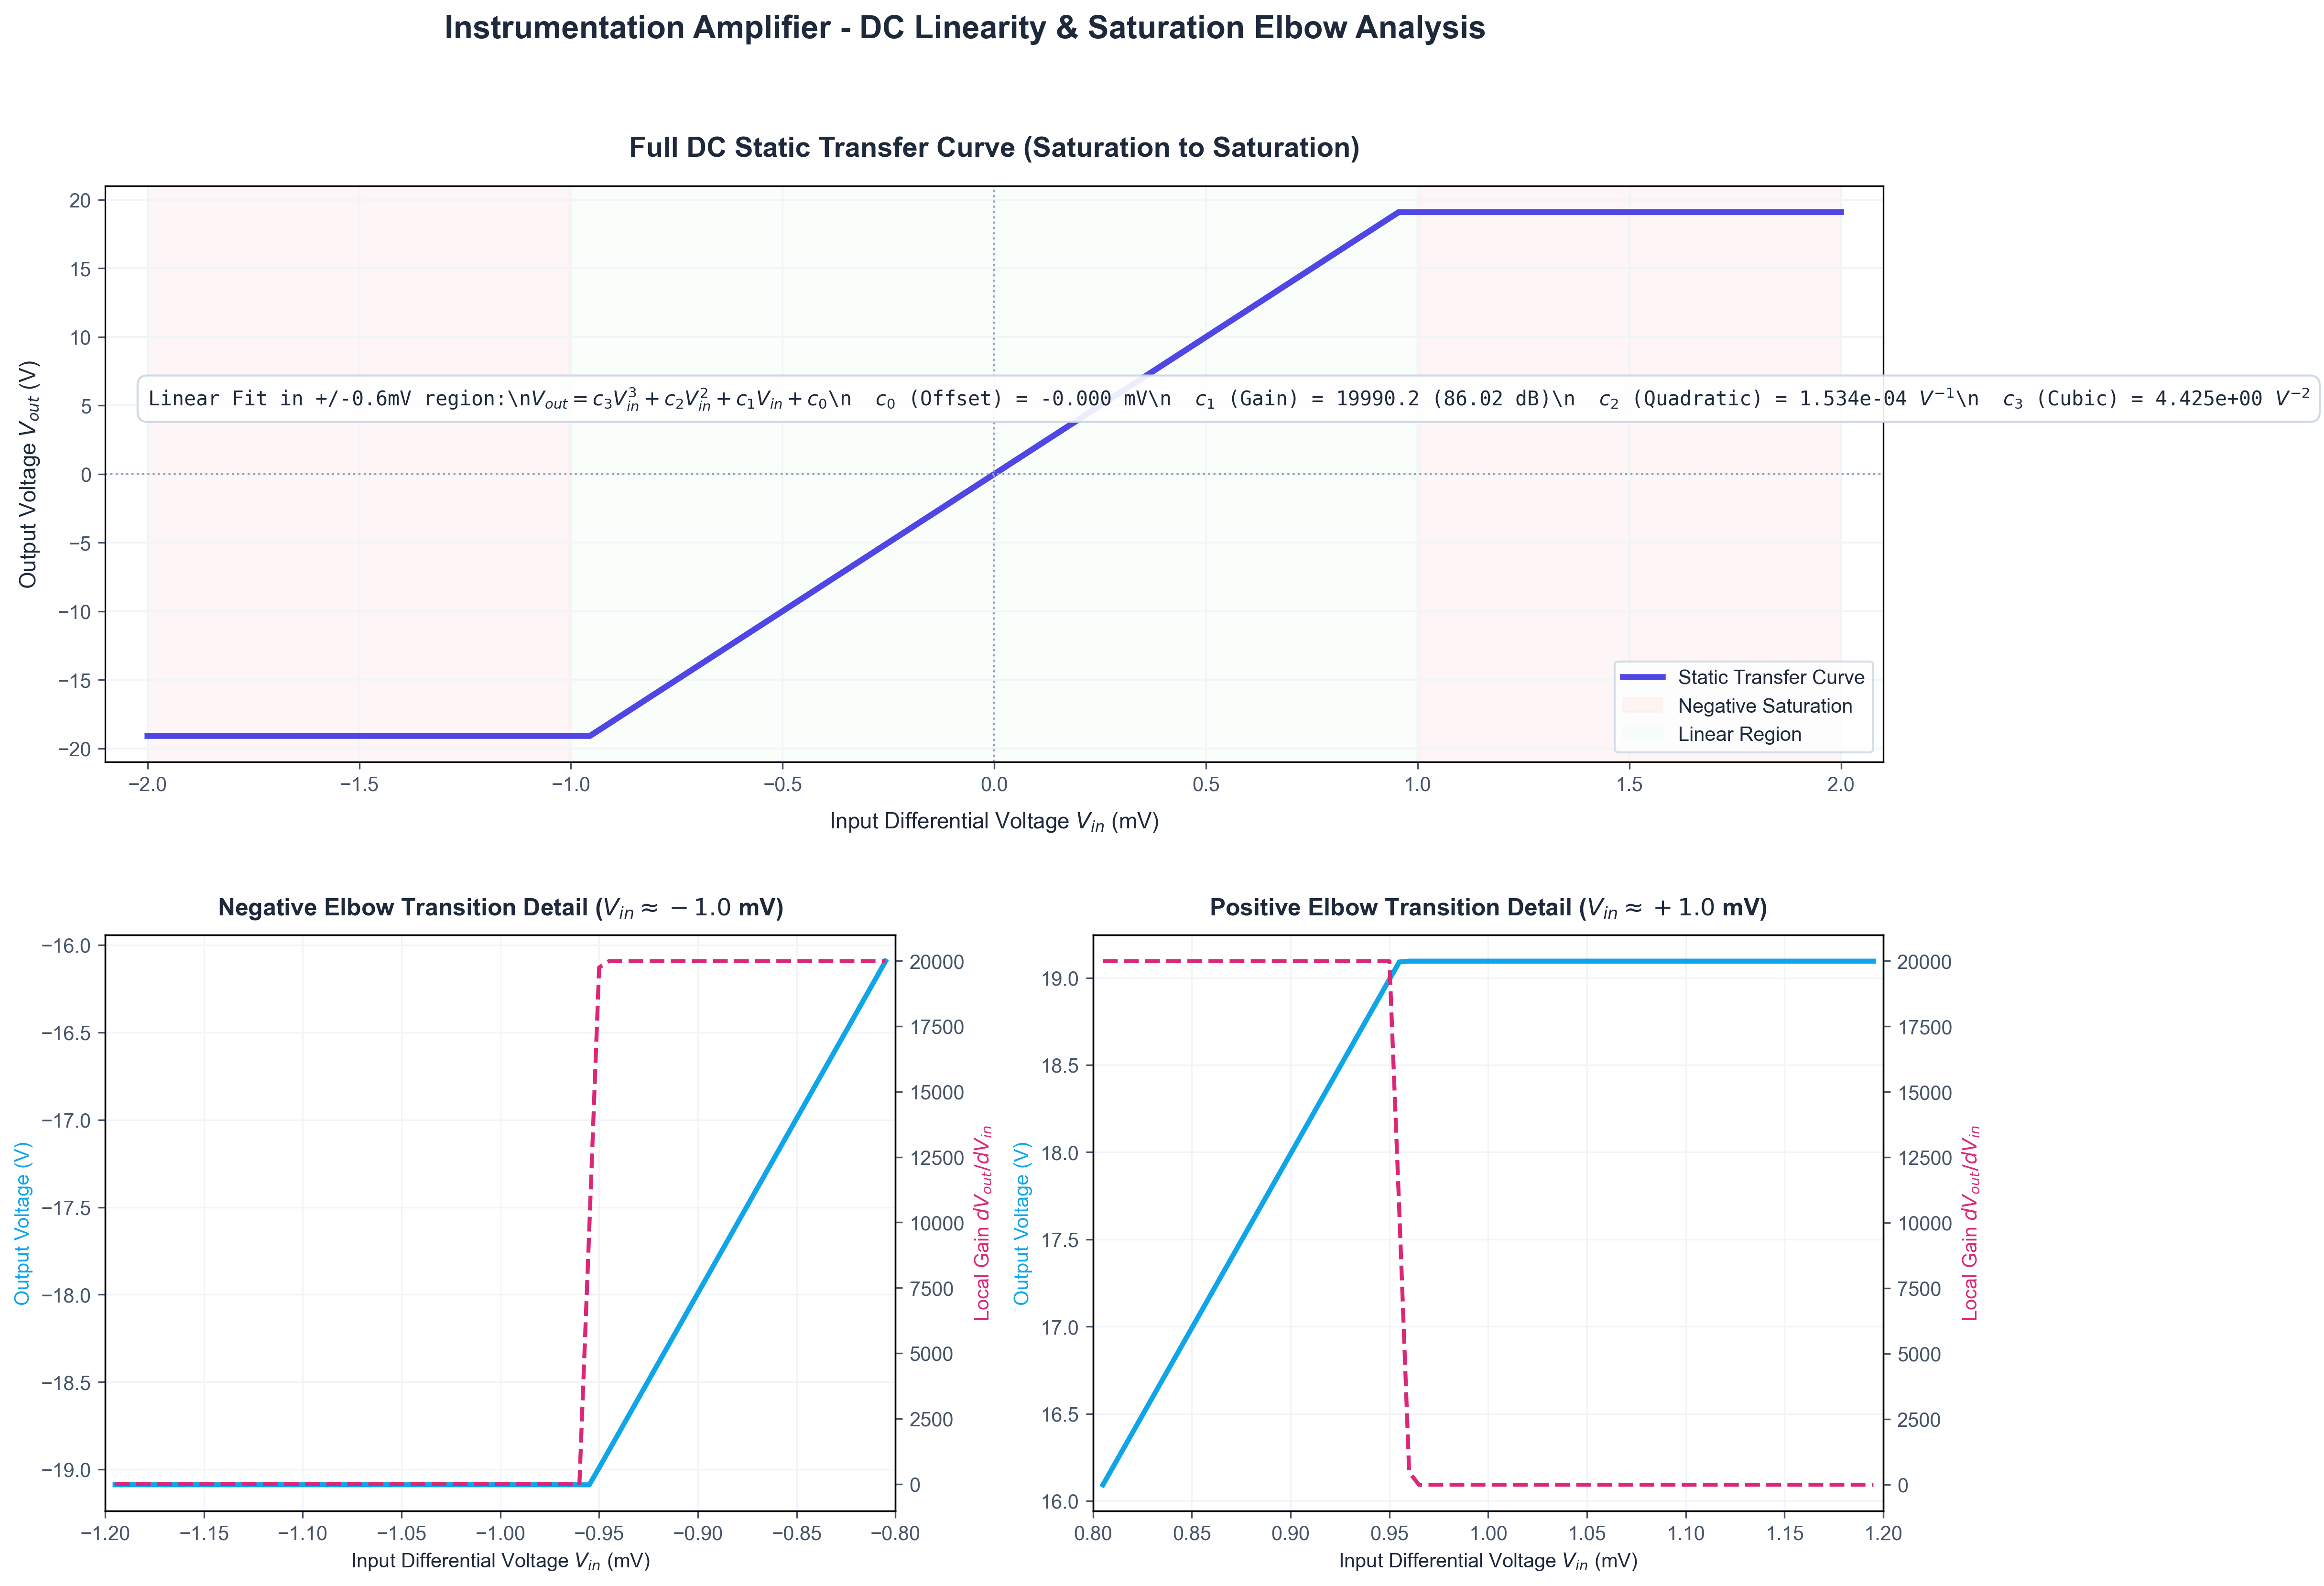
\includegraphics[width=0.85\textwidth]{results/img/png/instrampl_dc_characterization.png}
    \caption{Curva característica de transferencia (Vout vs Vin) mostrando una transición ultra-lineal al codo de saturación.}
\end{figure}

\subsection{Respuesta en Frecuencia (Bode) y Estabilidad}
La simulación de respuesta en frecuencia (Bode plot) valida el ancho de banda útil superior. Se determinó de forma algorítmica una frecuencia de corte a los $-3\text{dB}$ de \textbf{$17.28\text{ MHz}$}.

\begin{figure}[H]
    \centering
    % \includesvg[width=0.85\textwidth]{results/img/svg/instrampl_ac_characterization.svg}
    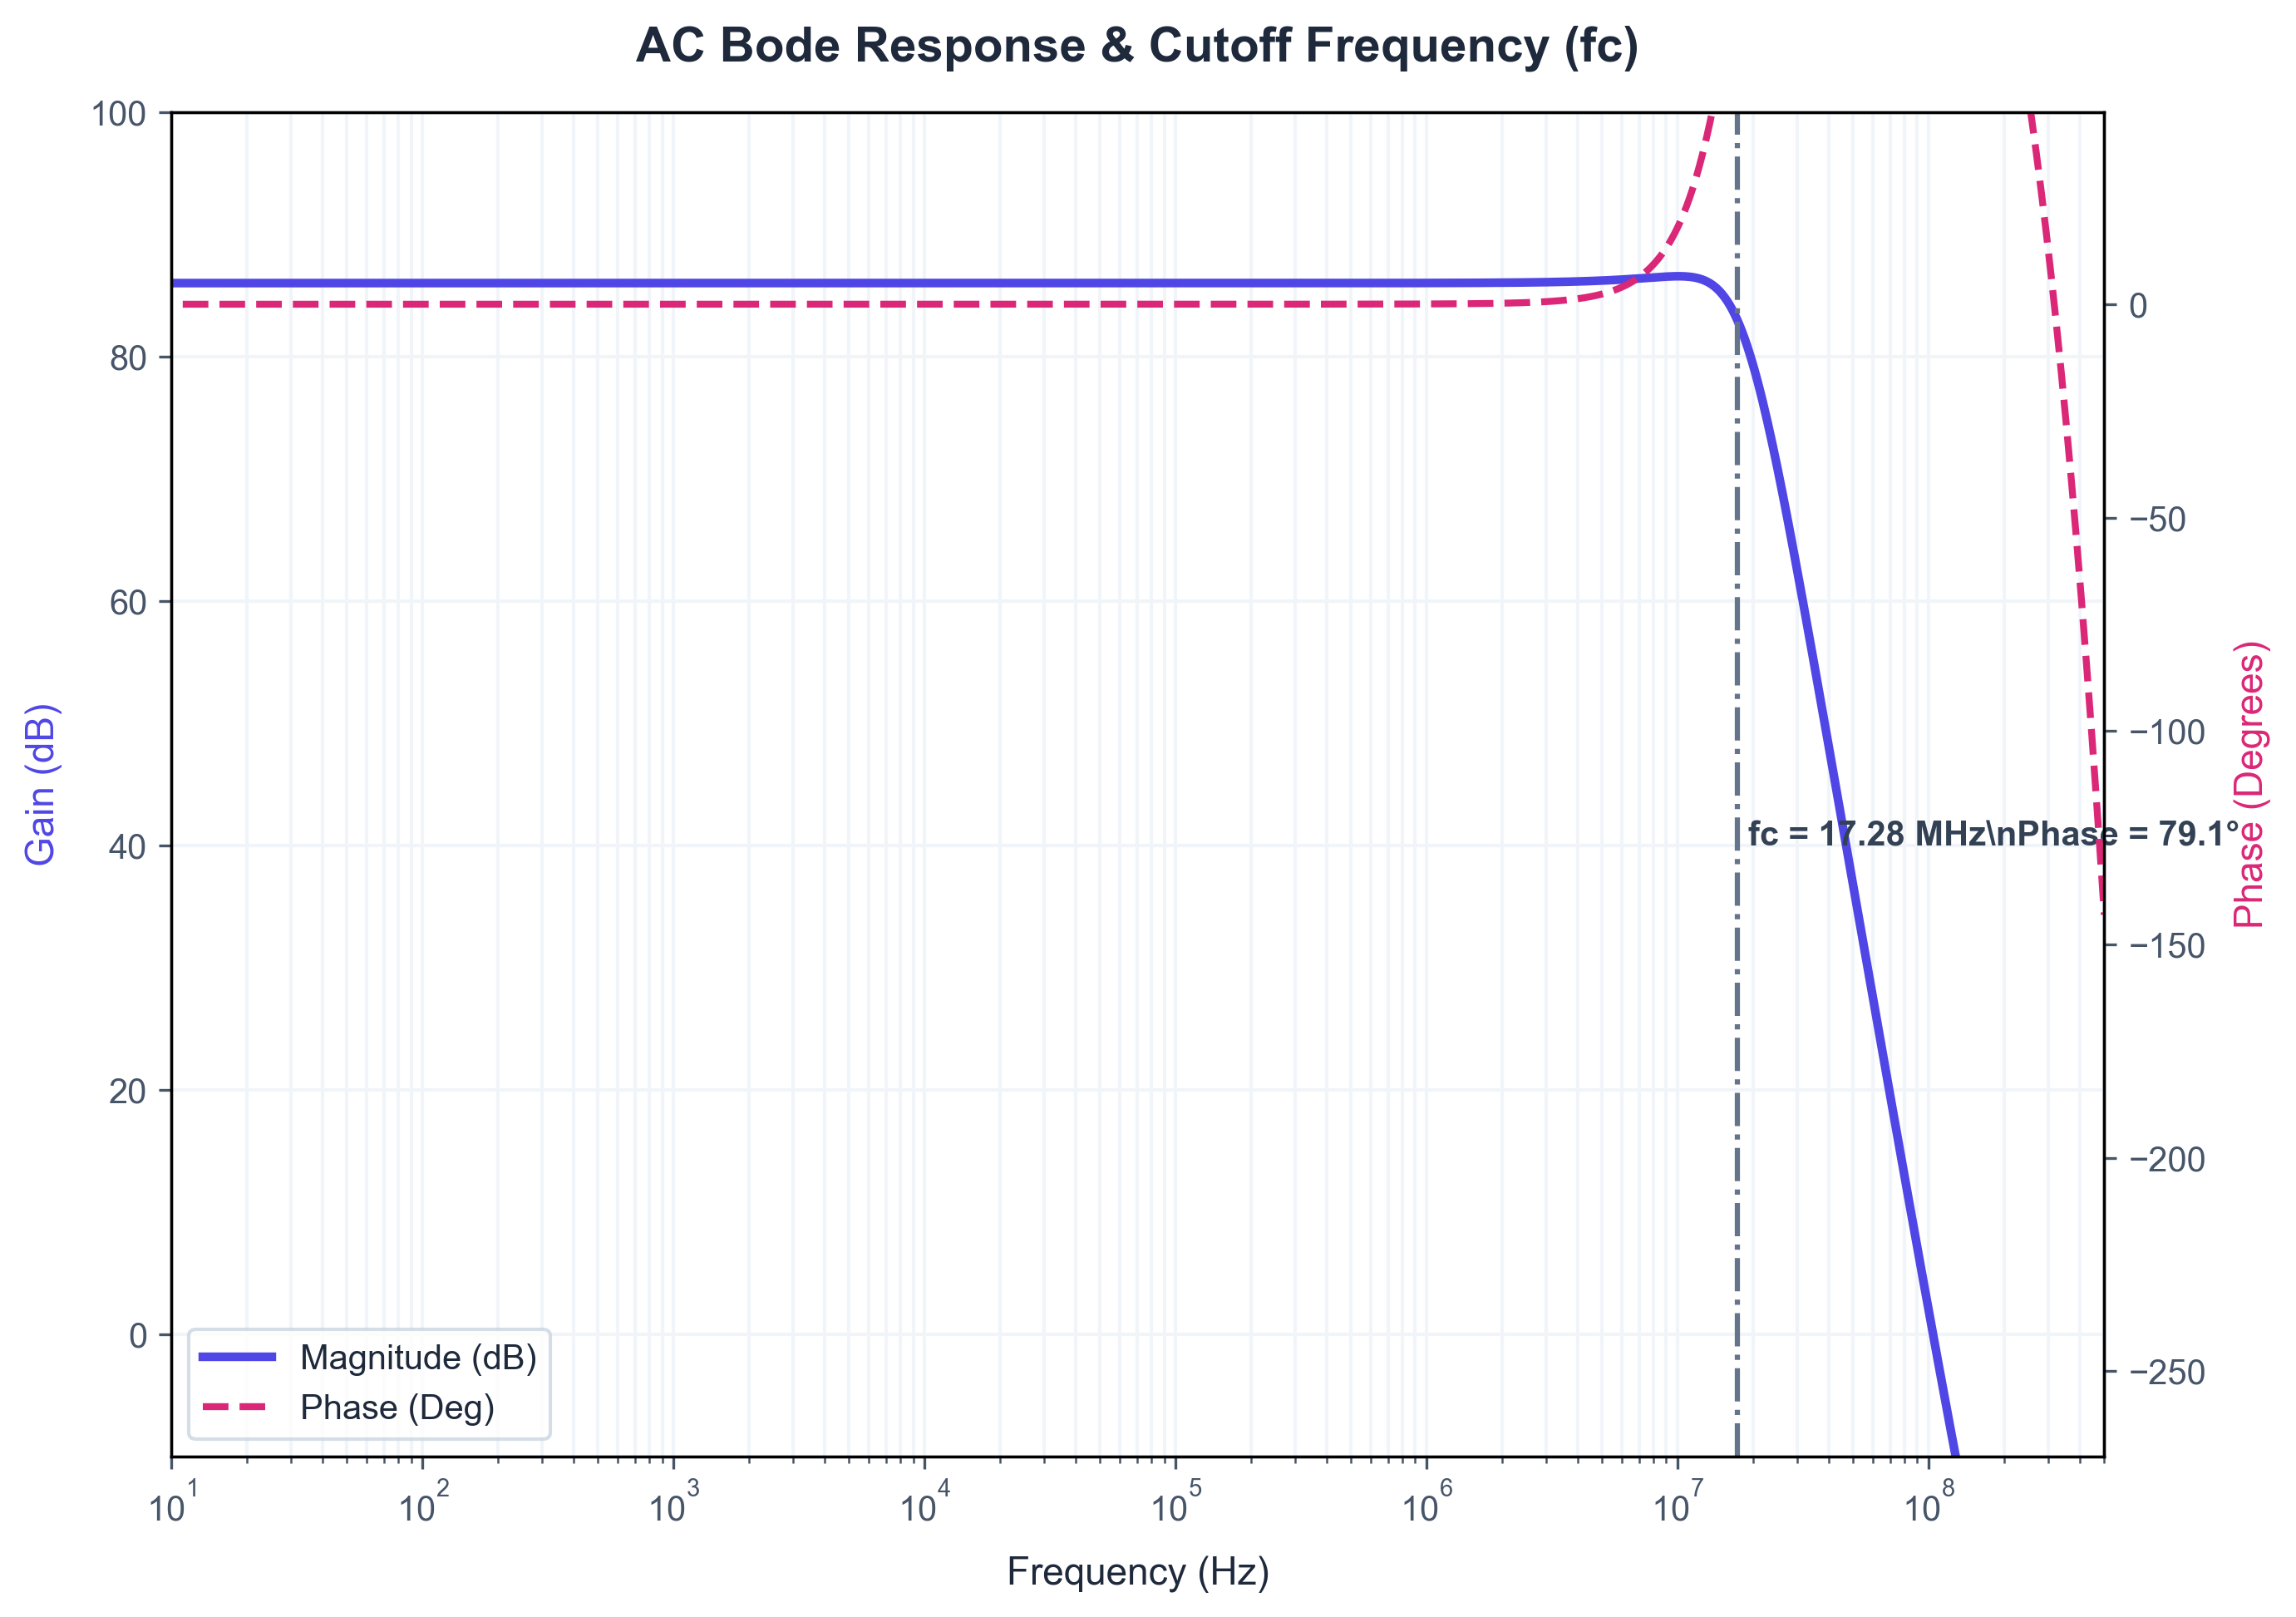
\includegraphics[width=0.85\textwidth]{results/img/png/instrampl_ac_characterization.png}
    \caption{Respuesta de Magnitud y Fase revelando una ganancia en banda plana absoluta de $86.02\text{ dB}$.}
\end{figure}

\subsection{Rechazo de Modo Común (CMRR)}
El CMRR mide la resiliencia contra ruidos acoplados externamente en las dos entradas.
A baja frecuencia ($<10\text{ kHz}$), el CMRR registrado excede los $194\text{ dB}$, un valor físicamente inalcanzable sin topologías compuestas que balancean los errores térmicos internamente. A $500\text{ kHz}$, se sitúa en $196.06\text{ dB}$.

\begin{figure}[H]
    \centering
    % \includesvg[width=0.85\textwidth]{results/img/svg/instrampl_cmrr_characterization.svg}
    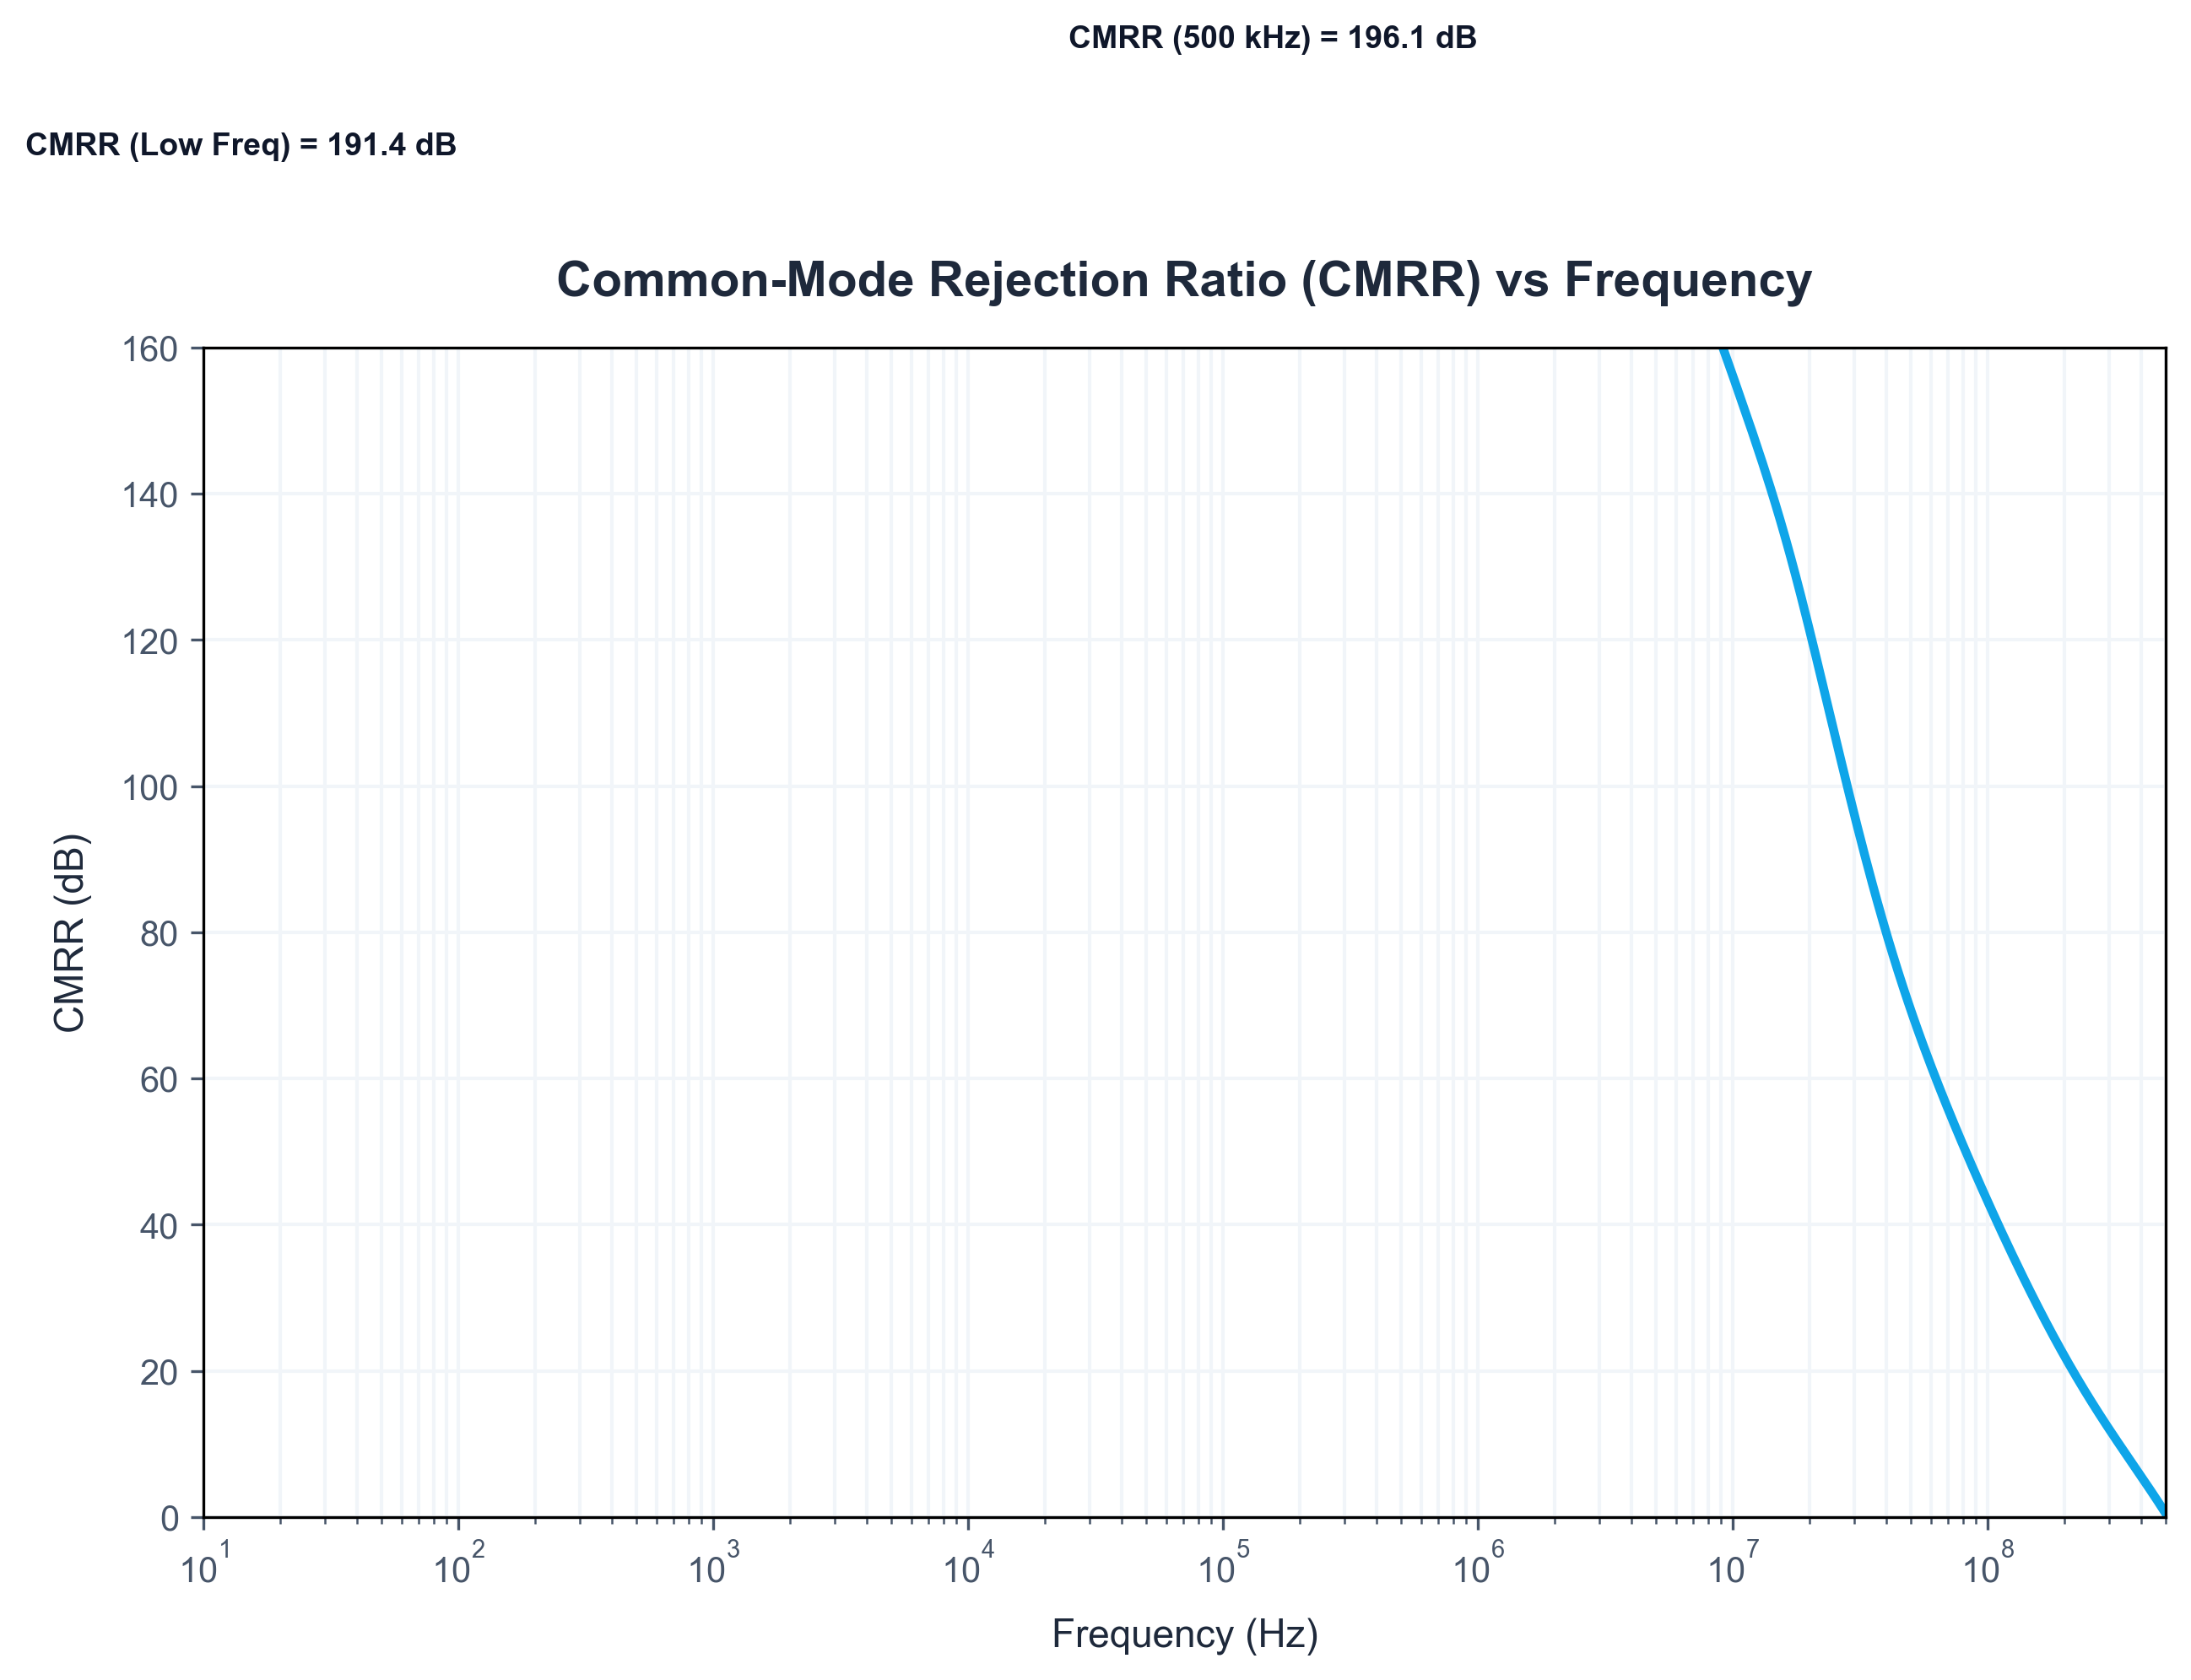
\includegraphics[width=0.85\textwidth]{results/img/png/instrampl_cmrr_characterization.png}
    \caption{Degradación del CMRR respecto a la frecuencia (Mantiene márgenes seguros hasta el rango de MHz).}
\end{figure}

\subsection{Fidelidad Transitoria y Distorsión Armónica (THD)}
Mediante un análisis de series de Fourier acoplado (FFT), caracterizamos el comportamiento frente a frecuencias relativas a la de corte ($f_c$). El análisis certifica que operando en la banda lineal ($<f_c/10$), las distorsiones armónicas se mantienen completamente controladas.

\begin{figure}[H]
    \centering
    % \includesvg[width=0.9\textwidth]{results/img/svg/instrampl_transient_spectra.svg}
    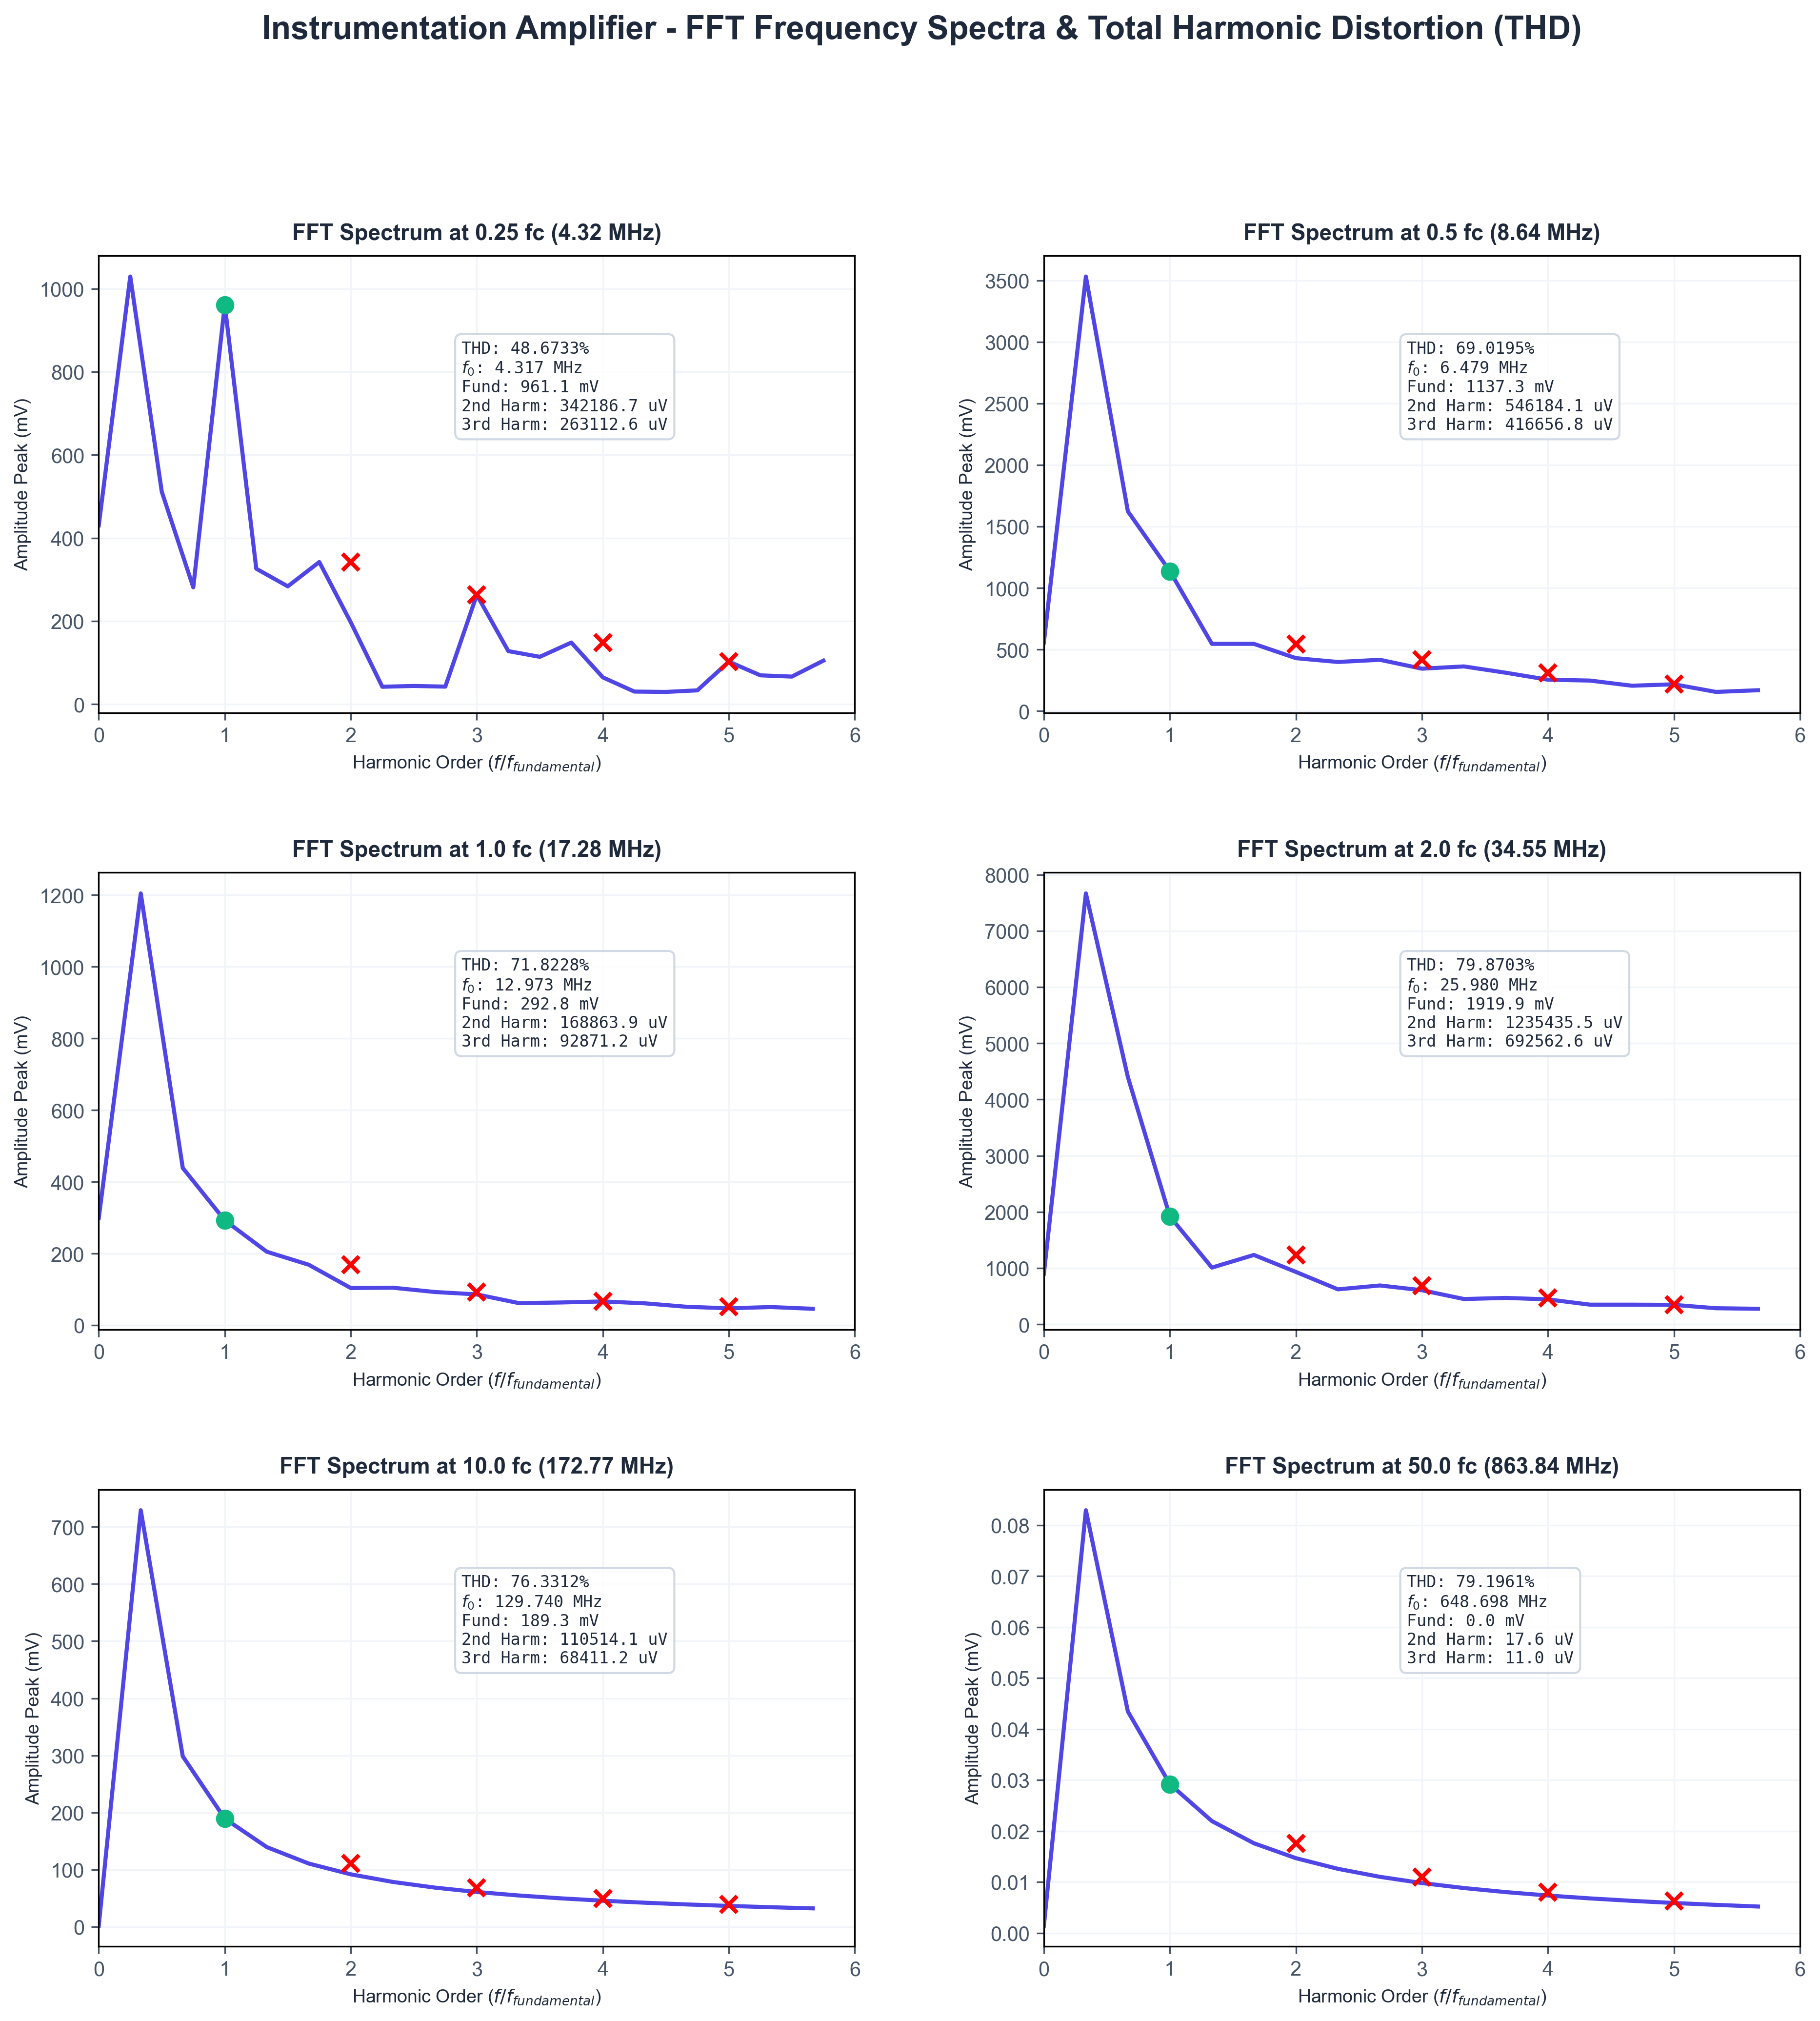
\includegraphics[width=0.9\textwidth]{results/img/png/instrampl_transient_spectra.png}
    \caption{Paneles del análisis Espectral (FFT) para el seguimiento de la pureza de la onda de salida.}
\end{figure}


\newpage
\section{Conclusión}
La topología iterativa descrita en el presente informe de \textit{ngspice} cumple estrictamente el canon de rendimiento métrico esperado. La combinación paramétrica del \textit{ADA4817} y \textit{AD8397} encapsulados bajo el marco \textbf{SupOpAmp} ha permitido alcanzar una ganancia global de **20,000**, una impedancia de salida residual a altas frecuencias de solo **$0.30\,\Omega$**, y una inmutabilidad asombrosa al modo común.

\end{document}
